\section{Sequencing}
\label{section:based-sequencer}

Utilizing the PBS model, a network of distinct builders and searchers emerges, 
engaging in competition to construct the most lucrative blocks that outbid others 
in the Realyer auction. L2 transactions adhere to a structure fully compatible with 
Ethereum, offering the potential to harness the capabilities of L1 builders and searchers. 
This approach enhances protocol stability and liveness while maintaining sovereignty. Refer 
to Figure \ref{figure:on-demand-design} for an illustration of the high-level schema.

\begin{figure}
    \centering
	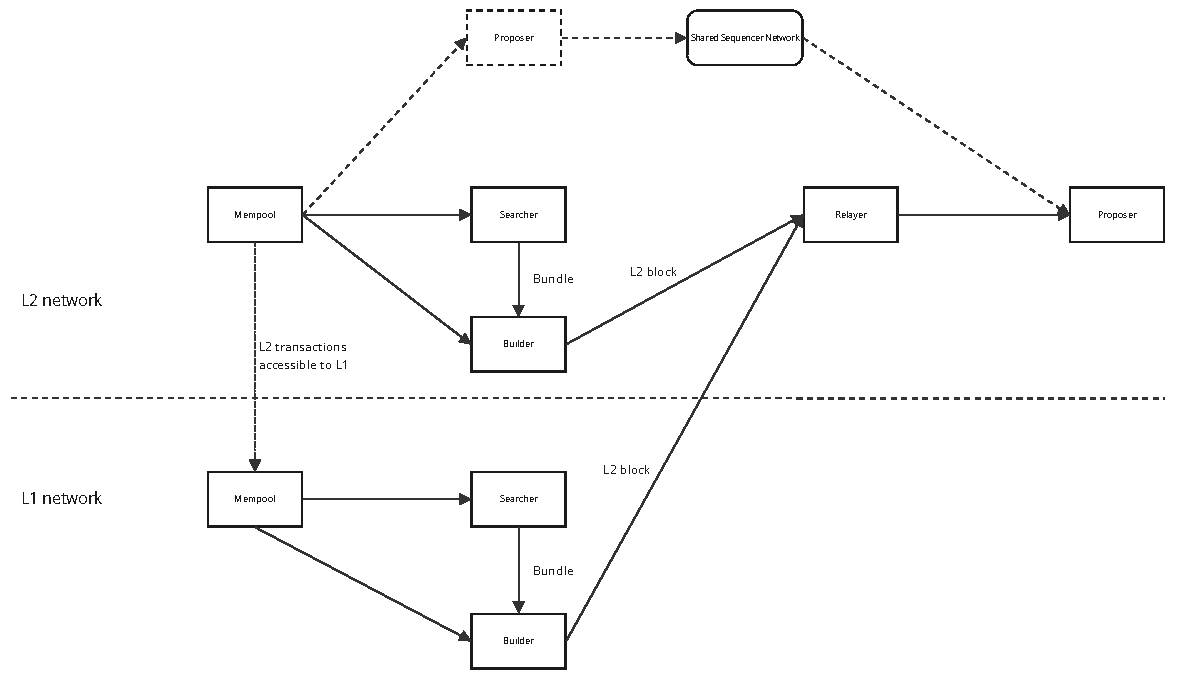
\includegraphics[scale=0.8]{figures/sequencer.pdf}
    \caption{Sequencing model}
     \label{figure:on-demand-design}
\end{figure}

\subsection{Shards' sequencing}


While each shard manages its own mempool of transactions, there are no restrictions on access 
for any network members. PBS participants have the autonomy to decide which shard to collaborate 
with. The associated risks that builders might choose to exclusively handle shards with high-gain 
applications (e.g., DeFi) are not significant. Several reasons substantiate the market stability 
of this model:

\begin{itemize}
    \item When numerous searchers and builders view to propose a single block to a relayer on a shard, 
    the likelihood of placing the highest bid with equivalent efficiency is directly proportional 
    to the number of effective builders. 
    The expected gain can be expressed as $E(G) = 1/n \cdot p$, where 
    n represents the number of effective builders and p is the expected gain.
    In the secondary shard with a lower gain, denoted as k, where the competition is less intense, the expected gain could 
    surpass that of the \mainshard in the case of smaller competition, i.e., $E(G_k) > E(G_n)$, 
    where $n < p/k$. 
    \\On the other side, gas prices rise for underloaded shards, and the gain $k$ will increase over time if the block 
    construction is delayed due to the inactivity of builders;
    \item A merge occurs when high gas prices result from the inactivity of builders.
\end{itemize}

Following the principle of PBS and a separated mempool, the possibility arises to utilize 
independent sequencers tailored to specific needs. 
The integration and utilization are seamlessly designed, 
 allowing validators to choose such a system over independent builders 
 to enhance specific aspects of the shard.
For instance, reducing MEV on a shard with a highly liquid decentralized exchange could potentially significantly decrease slippage, 
 although not mandatory, but likely increasing transaction costs. 
An example of this integration is illustrated in Figure \ref{figure:on-demand-design} (dotted line).

% \begin{remark}
%     Split and merge events can represent a significant shift for builders and searchers.
%     Any changes to the entire network, including the involved members, will be communicated 
%     through the \mainshard.
%     In practice, without maintaining a long queue of pre-prepared blocks, 
%     the merge event will not introduce significant changes to the constructed builder's blocks 
%     (e.g., shardID). 
%     Relayers will need to reapprove signatures in the new committee after the 
%     event to continue delivering blocks to the proposers.
% \end{remark}

\subsection{\mainshard}

The \mainshard distinguishes itself from others with its essential requirements of speed and 
liveness. However, a set of associated risks has emerged along with the reasons for their 
association:
\begin{itemize}
    \item No potential MEV issues, due to specifics of the transactions.
    \item No market competition for gas prices due to exclusivity.
    \item With few shards quite a lot of unutilized block gas.
\end{itemize}

This requires an approach where proposers both construct and verify blocks, eliminating the 
need for a separate role. Instead, a committee will oversee the construction process, and 
transaction costs will be covered by the protocol fee. The estimation of gas prices for the 
\mainshard is derived from the market price.